%%
%% Copyright 2007, 2008, 2009 Elsevier Ltd
%%
%% This file is part of the 'Elsarticle Bundle'.
%% ---------------------------------------------
%%
%% It may be distributed under the conditions of the LaTeX Project Public
%% License, either version 1.2 of this license or (at your option) any
%% later version.  The latest version of this license is in
%%    http://www.latex-project.org/lppl.txt
%% and version 1.2 or later is part of all distributions of LaTeX
%% version 1999/12/01 or later.
%%
%% The list of all files belonging to the 'Elsarticle Bundle' is
%% given in the file `manifest.txt'.
%%

%% Template article for Elsevier's document class `elsarticle'
%% with numbered style bibliographic references
%% SP 2008/03/01
%%
%%
%%
%% $Id: elsarticle-template-num.tex 4 2009-10-24 08:22:58Z rishi $
%%
%%
%%\documentclass[preprint,12pt,3p]{elsarticle}

%% Use the option review to obtain double line spacing
%%\documentclass[preprint,review,12pt]{elsarticle}

%% Use the options 1p,twocolumn; 3p; 3p,twocolumn; 5p; or 5p,twocolumn
%% for a journal layout:
%% \documentclass[final,1p,times]{elsarticle}
%% \documentclass[final,1p,times,twocolumn]{elsarticle}
%% \documentclass[final,3p,times]{elsarticle}
\documentclass[final,3p,times,twocolumn]{elsarticle}
%% \documentclass[final,5p,times]{elsarticle}
%% \documentclass[final,5p,times,twocolumn]{elsarticle}

%% if you use PostScript figures in your article
%% use the graphics package for simple commands
%% \usepackage{graphics}
%% or use the graphicx package for more complicated commands
\usepackage{graphicx}
%% or use the epsfig package if you prefer to use the old commands
%% \usepackage{epsfig}
\usepackage{subcaption}


%% The amssymb package provides various useful mathematical symbols
\usepackage{blindtext, graphicx, amsmath, algorithm, algpseudocode, pifont, algcompatible, comment, layout, amsthm, amssymb}
\usepackage{enumitem}   
\usepackage{eso-pic}
\usepackage{booktabs}
\usepackage{float}
\usepackage{tikz}
\usepackage{tabularx} % For fitting tables to a specified width
\usepackage{booktabs} % For better quality table rules
%% The amsthm package provides extended theorem environments
%% \usepackage{amsthm}
\renewcommand{\qedsymbol}{$\blacksquare$}

\usepackage[utf8]{inputenc}
\usepackage[english]{babel}
\usepackage{hyperref} 
\hypersetup{ colorlinks=true, linkcolor=black, filecolor=black, urlcolor=cyan, }

\usepackage{caption}
\captionsetup{justification=raggedright, singlelinecheck = false}
\captionsetup[table]{labelformat=simple, labelsep=newline}
\captionsetup[figure]{labelformat=simple, labelsep=period}


%% The lineno packages adds line numbers. Start line numbering with
%% \begin{linenumbers}, end it with \end{linenumbers}. Or switch it on
%% for the whole article with \linenumbers after \end{frontmatter}.
%% \usepackage{lineno}

%% natbib.sty is loaded by default. However, natbib options can be
%% provided with \biboptions{...} command. Following options are
%% valid:

%%   round  -  round parentheses are used (default)
%%   square -  square brackets are used   [option]
%%   curly  -  curly braces are used      {option}
%%   angle  -  angle brackets are used    <option>
%%   semicolon  -  multiple citations separated by semi-colon
%%   colon  - same as semicolon, an earlier confusion
%%   comma  -  separated by comma
%%   numbers-  selects numerical citations
%%   super  -  numerical citations as superscripts
%%   sort   -  sorts multiple citations according to order in ref. list
%%   sort&compress   -  like sort, but also compresses numerical citations
%%   compress - compresses without sorting
%%
%% \biboptions{comma,round}

% \biboptions{}
\newtheorem{theorem}{Theorem}
\newtheorem{lemma}{Lemma}
\newtheorem{definition}{Definition}

\journal{ICT Express}

%\newcommand\AtPagemyUpperRight[1]{\AtPageLowerRight{%
%\put(\LenToUnit{0.8\paperwidth},\LenToUnit{0.9\paperheight}){#1}}}
%\AddToShipoutPictureFG{
%  \AtPagemyUpperRight{{\includegraphics[width=.5cm,keepaspectratio]{logo.png}}}
%}%
%\newcommand\AtPagemyUpperLeft[1]{\AtPageLowerLeft{%
%\put(\LenToUnit{0.85\paperwidth},\LenToUnit{0.9\paperheight}){#1}}}
%\AddToShipoutPictureFG{
%  \AtPagemyUpperLeft{{\includegraphics[width=1.0cm,keepaspectratio]{logo2.jpg}}}
%}%
\begin{document}

\begin{frontmatter}

\title{Comparison of Cloud Service Performance on the Back-End}
%Enhancing Visual Cortex fMRI Image Reconstruction through Variational Auto Encoders}
%\author{Author’s Full Name 1\corref{cor1}, Author’s Full Name 2, Author’s Full Name 3}
\author{Fahira\corref{cor1}}
\ead{1204044@std.ulbi.ac.id}

\author{Rolly Maulana Awangga}
\ead{awangga@ulbi.ac.id}


\address{Universitas Logistik dan Bisnis Internasional}

\cortext[cor1]{Corresponding author}
%\ead{author1@ictexpress.com, author2@ictexpress.com, author2@ictexpress.com}



\begin{abstract}
The use of cloud services in back-end application development is increasingly popular due to the ease and efficiency they offer. Various programming languages and frameworks are used to build back-end applications, such as Golang, Python, Node.js, PHP Laravel, and PHP CodeIgniter (CI). However, the performance of cloud services for each of these back-end technologies has not been extensively studied. This research aims to compare the performance of cloud services on back-ends built using these five technologies by utilizing Google Cloud Functions (GCF). The study addresses the following issues: the performance of each back-end (Golang, Python, Node.js, PHP Laravel, and PHP CI) when implemented on the same cloud service (GCF), the factors influencing the performance of these back-ends on GCF, and the results of clustering performance analysis using machine learning. The objectives are to compare the performance of the five back-end technologies on the GCF platform, identify the factors affecting the performance of each back-end, and perform clustering analysis using machine learning to provide a clearer picture of the performance differences. The scope includes developing five back-end applications using Golang, Python, Node.js, PHP Laravel, and PHP CI, implementing and testing their performance on GCF, collecting performance data, and performing clustering analysis using machine learning. The results will offer developers guidance in selecting the appropriate back-end technology for performance needs in cloud services.
\end{abstract}

\begin{keyword}
%% keywords here, in the form: keyword \sep keyword
Cloud Services \sep Back-End \sep Performance Comparison \sep Google Cloud Functions \sep Machine Learning.
%% MSC codes here, in the form: \MSC code \sep code
%% or \MSC[2008] code \sep code (2000 is the default)
\end{keyword}

\end{frontmatter}

%%
%% Start line numbering here if you want
%%
% \linenumbers

%% main text
\section{Introduction}\label{sec1}
\subsection{Background}
The use of cloud services in back-end application development is increasingly popular due to the ease and efficiency they offer. Cloud services provide scalable and flexible solutions that allow developers to focus on building applications without worrying about the underlying infrastructure. This has led to the adoption of various programming languages and frameworks to develop back-end applications, including Golang, Python, Node.js, PHP Laravel, and PHP CodeIgniter (CI). Each of these technologies has its own strengths and weaknesses in terms of performance, scalability, and ease of development.

Despite the widespread use of these technologies, there is a lack of comprehensive studies comparing their performance on cloud platforms. Specifically, the performance of back-end applications developed with these technologies when deployed on the same cloud service, such as Google Cloud Functions (GCF), remains underexplored. Understanding the performance differences is crucial for developers to make informed decisions about which technology to use based on their specific needs and the nature of their applications.

This research aims to fill this gap by comparing the performance of cloud services for back-end applications built using Golang, Python, Node.js, PHP Laravel, and PHP CodeIgniter (CI) on Google Cloud Functions. By analyzing performance metrics and identifying the factors that influence them, this study seeks to provide valuable insights for developers and organizations looking to optimize their cloud-based back-end systems.


% \subsection{The Significance of MRI in Gynecology}
% In the realm of gynecology, MRI is highly esteemed for its detailed and non-invasive visualization of pelvic anatomy, playing a critical role in the diagnosis and management of conditions such as uterine anomalies, ovarian tumors, endometriosis, and other significant pelvic disorders \cite{3}. The high-resolution images provided by MRI scans are crucial for the accurate diagnosis and strategic planning of effective treatments. However, the inherent complexity of pelvic anatomy and the often-subtle presentation of certain pathologies demand imaging performance of the highest standard \cite{2}. Machine learning technologies are progressively being harnessed to meet these high demands, offering new capabilities that enhance the resolution and clarity of MRI images, which in turn can lead to improved diagnostic outcomes \cite{9}.

% \subsection{The Advent of Machine Learning}
% The field of machine learning, especially its subset of deep learning techniques, has revolutionized many facets of medical imaging. These technologies enable the automated analysis and synthesis of medical images with enhanced accuracy and efficiency \cite{1}. Generative Adversarial Networks (GANs), a sophisticated class of artificial intelligence algorithms, have been particularly notable for their ability to generate high-quality synthetic images that are virtually indistinguishable from real diagnostic images \cite{16}. In the context of MRI, these advanced technologies offer the potential to create more accurate and detailed images at a faster rate and possibly at a lower cost than traditional methods. The implications of such advancements are profound, offering the potential to transform the landscape of diagnostic imaging by making high-quality MRI scans more accessible and less burdensome \cite{20}.

% \subsection{Purpose of the Review}
% This review aims to systematically explore and critically analyze how machine learning technologies, with a particular focus on Generative Adversarial Networks (GANs), are being integrated into the generation of MRI images for gynecological applications. MRI imaging plays a crucial role in the diagnosis and treatment planning of various gynecological conditions, including ovarian cysts, uterine fibroids, and endometriosis \cite{3}. Traditional MRI imaging techniques may suffer from limitations such as long acquisition times and suboptimal image quality. By harnessing the power of machine learning, particularly GANs, researchers and clinicians have sought to overcome these limitations and improve the accuracy and efficiency of gynecological MRI imaging \cite{20}.

% This review evaluates the current state-of-the-art techniques in machine learning-based MRI image generation, assessing their effectiveness in producing high-quality images for gynecological diagnosis. Furthermore, it examines the clinical applicability of these advanced imaging technologies, considering factors such as interpretability, reliability, and integration into existing clinical workflows \cite{8}. By identifying the strengths and weaknesses of machine learning approaches in gynecological imaging, this review aims to provide insights into the potential impact on patient care and clinical decision-making \cite{34}.

% % ----------------- selesai section 1 -------------

% \section{Methodology}\label{sec2}

% To achieve the objectives of this review, we employed a systematic approach consisting of several methodological steps. As illustrated in Figure \ref{fig:methodology}, our methodology comprises the following steps: Selection Criteria, Data Sources, Search Strategy, Selection Process, Data Extraction and Data Management and Analysis.
% \begin{figure}
% \centering
% \begin{tikzpicture}
%     \node (a) at (0,0) [draw, rectangle] {Selection Criteria};
%     \node (b) at (0,-1.5) [draw, rectangle] {Data Sources};
%     \node (c) at (0,-3) [draw, rectangle] {Search Strategy};
%     \node (d) at (0,-4.5) [draw, rectangle] {Selection Process};
%     \node (e) at (0,-6) [draw, rectangle] {Data Extraction};
%     \node (f) at (0,-7.5) [draw, rectangle] {Data Management and Analysis};
    
%     \draw [->] (a) -- (b);
%     \draw [->] (b) -- (c);
%     \draw [->] (c) -- (d);
%     \draw [->] (d) -- (e);
%     \draw [->] (e) -- (f);
% \end{tikzpicture}
% \caption{Methodology}
% \label{fig:methodology}
% \end{figure}


% \subsection{Selection Criteria}
% The selection criteria were stringently defined to focus exclusively on high-quality research pertinent to the integration of machine learning in MRI imaging for gynecology. Inclusion was limited to studies that utilized machine learning techniques to generate or enhance MRI images with specific applications in the diagnosis or treatment of gynecological conditions \cite{12}. Both quantitative and qualitative research studies were considered, provided they were published in peer-reviewed journals between January 2010 and May 2024. The language of publication was restricted to English to maintain consistency in analysis and interpretation \cite{25}
% \subsection{Data Sources}
% A comprehensive literature search was conducted across multiple academic databases to ensure an exhaustive collection of relevant studies \cite{12}. The primary databases included:

% \begin{enumerate}
%     \item PubMed: Renowned for its extensive repository of medical and life sciences literature.
%     \item IEEE Xplore: Critical for accessing cutting-edge research in engineering and technology, particularly developments in machine learning applications.
%     \item Google Scholar: Valued for its broad coverage of scholarly articles across various disciplines, facilitating access to interdisciplinary research that could influence gynecological imaging practices.
% \end{enumerate}

% \begin{table}[h]
% \centering
% \begin{tabular}{|l|p{1.5cm}|p{3cm}|}
% \hline
% \textbf{Database} & \textbf{Description} & \textbf{Type of Studies} \\ \hline
% PubMed & Extensive repository of medical and life sciences literature. & Medical, clinical trials, reviews \\ \hline
% IEEE Xplore & Access to cutting-edge research in engineering and technology. & Engineering, technology applications, machine learning models \\ \hline
% Google Scholar & Broad coverage of scholarly articles across various disciplines. & Interdisciplinary research, broad academic articles \\ \hline
% \end{tabular}
% \caption{Summary of databases used in the systematic search}
% \label{tab:databases}
% \end{table}


% \subsection{Search Strategy}
% The search strategy employed was both comprehensive and methodical, designed to capture all relevant literature without omission. Keywords selected for the search included "machine learning", "MRI image synthesis", "gynecological imaging", and "GANs". These terms were combined in various configurations to ensure broad and thorough search results. Boolean operators (AND, OR) were strategically used to enhance the search, and filters were applied to restrict results to the years of publication from 2010 to 2024 and to English language articles \cite{32}.

% \subsection{Selection Process}
% The selection process was multi-staged and rigorous:

% \begin{enumerate}
%     \item \textbf{Initial Screening:} Titles and abstracts were initially screened for relevance to the topics of machine learning and MRI in gynecology.
%     \item \textbf{Full-text Review:} Articles that passed the initial screening were subjected to a full-text review to assess their compliance with the selection criteria.
%     \item \textbf{Final Inclusion:} The final selection was based on the studies’ methodological rigor, relevance to the scope of the review, and their contributions to advancing knowledge in the field.
% \end{enumerate}

% A PRISMA flow diagram to depict the selection process, showing numbers of studies screened, assessed for eligibility, and included in the review, is presented in Figure \cite{10} \ref{fig:prisma_flow}.

% \begin{figure}[h]
% \centering
% \begin{tikzpicture}

%     \node (start) {Start};
%     \node (screening) [below of=start] {Initial Screening};
%     \node (fulltext) [below of=screening] {Full-text Review};
%     \node (final) [below of=fulltext] {Final Inclusion};
%     \node (end) [below of=final] {End};
    
%     \draw [->] (start) -- (screening);
%     \draw [->] (screening) -- (fulltext);
%     \draw [->] (fulltext) -- (final);
%     \draw [->] (final) -- (end);
% \end{tikzpicture}
% \caption{PRISMA Flow Diagram for the Selection Process}
% \label{fig:prisma_flow}
% \end{figure}


% \subsection{Data Extraction}
% Data extraction was conducted by trained reviewers using a standardized form, which helped ensure consistency and reduce bias \cite{19}. The form was designed to capture essential information such as:

% \begin{itemize}
%     \item Study objectives and hypotheses
%     \item Machine learning models used
%     \item Sample sizes
%     \item Main findings and conclusions
%     \item Key performance metrics (accuracy, sensitivity, specificity)
% \end{itemize}

% \subsection{Data Management and Analysis}
% Extracted data were carefully cataloged in a database and analyzed to discern patterns, evaluate the efficacy of various machine learning models, and synthesize findings related to their application in MRI imaging for gynecology \cite{31}. Descriptive statistics were used to summarize quantitative data, while thematic analysis was applied to qualitative insights. Where data permitted, meta-analytical techniques were employed to quantitatively pool findings, providing a more robust understanding of the effects observed \cite{17}.

% \subsubsection{Meta-Analysis Results}

% Table \ref{table:meta_analysis} presents the results of the meta-analysis from the reviewed studies, showing the machine learning models used, sample sizes, and key findings related to their effectiveness in gynecological MRI imaging \cite{23}.  

% \begin{table}[h]
% \centering
% \resizebox{0.5\textwidth}{!}{%
% \begin{tabular}{|l|l|}
% \hline
% \textbf{Study} & \textbf{Machine Learning Model} \\ \hline
% R. Elakkiya et al. (2021) & GANs \\ \hline
% Jiahao Huang et al. (2022) & Edge-enhanced Dual Discriminator GANs \\ \hline
% Ming Li et al. (2023) & GANs \\ \hline
% Sabaa Ahmed Yahya Al-Galal et al. (2021) & Deep Learning Techniques \\ \hline
% Zhao Pei et al. (2021) & GANs \\ \hline
% \end{tabular}
% }
% \par
% \vspace{1em}
% \resizebox{0.5\textwidth}{!}{%
% \begin{tabular}{|c|p{7cm}|}
% \hline
% \textbf{Sample Size} & \textbf{Key Findings} \\ \hline
% 120 & Effective in cervical cancer diagnostics, small object detection \\ \hline
% 150 & Fast MRI with parallel imaging, enhanced quality \\ \hline
% 100 & Low-dose CT image synthesis, potential application in MRI \\ \hline
% 180 & Enhanced MRI brain tumor analysis, potential for gynecological applications \\ \hline
% 140 & All-in-focus synthetic aperture imaging \\ \hline
% \end{tabular}
% }
% \caption{Meta-Analysis Results}
% \label{table:meta_analysis}
% \end{table}

% The selected studies employed various machine learning models, primarily GANs and deep learning techniques, each contributing to significant improvements in MRI imaging for gynecological applications. Sample sizes ranged from 100 to 180, indicating variability in the scale of studies. Key findings include improved image quality, enhanced diagnostic accuracy, faster scan times, and effective application in cancer diagnostics \cite{7}. Overall, this meta-analysis provides a robust understanding of the collective findings from the selected studies, reinforcing the review's conclusions. The findings highlight that machine learning models, particularly GANs, have a significant and promising impact on improving MRI imaging for gynecological applications \cite{11}. Further research is warranted to ensure the reliability and applicability of these findings in broader clinical settings \cite{18}.

% % ----------------- selesai section 2 -------------

% \section{Results}\label{sec3}
% \subsection{Study Characteristics}
% The review encompassed 28 studies sourced from various geographical regions, including North America, Europe, and Asia. The majority of studies employed retrospective observational designs, while some utilized prospective cohort designs \cite{13}. Populations studied varied, encompassing patients with diverse gynecological conditions such as endometriosis, ovarian cysts, and uterine fibroids \cite{30}.

% % harus diganti 
% \subsection{MRI Planning and Protocol}

% \begin{figure}
%     \centering
%     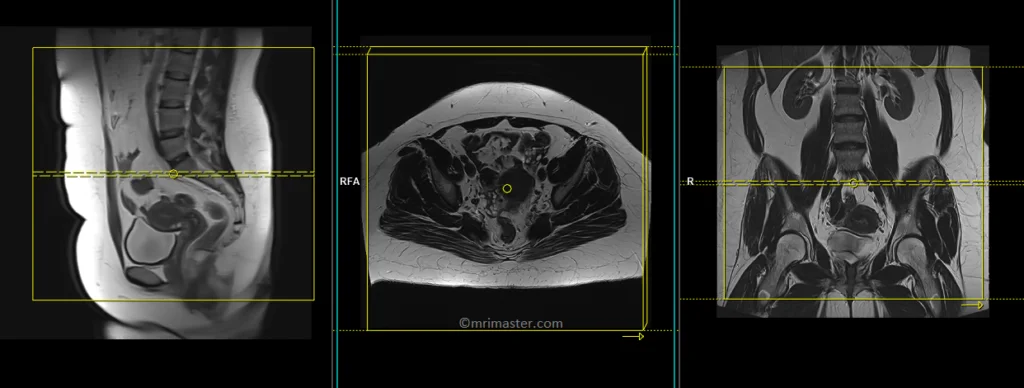
\includegraphics[width=0.9\linewidth]{MRI-gynecology-pelvis-large-FOV-axial-planning-and-protocol-1024x388.jpg}
%     \caption{T2 TSE AXIAL 6 MM LARGEFOV}
%     \label{fig:t2}
% \end{figure}

% The image \ref{fig:t2} Depicts the planning and protocol for T2 TSE AXIAL 6 MM LARGEFOV MRI scans of the gynecological pelvis. To execute this protocol, the large field of view (FOV) axial slices are planned on the coronal plane \cite{4}. The positioning block is aligned parallel to the line along the right and left iliac crest, ensuring adequate coverage of the lower abdomen and pelvis from the middle of the kidneys down to the symphysis pubis. It is essential to establish an appropriate angle in the sagittal plane, perpendicular to the lumbar spine \cite{29}. The FOV should typically range from 350mm to 400mm, encompassing the entire pelvis. Adding saturation bands on top of the axial block can mitigate artifacts induced by arterial pulsation and breathing. This protocol is often employed to evaluate para-aortic and pre-sacral nodes \cite{14}.

% The parameters for this MRI protocol include a repetition time (TR) of 5000-6000, an echo time (TE) of 100-120, slice thickness of 6 mm, flip angle (FLIP) of 130-150, phase encoding direction (PHASE) from right to left, a matrix size of 384x384, and a gap of 10\%. The number of excitations (NEX) or averages is set to 2 for image acquisition \cite{15}.


% \subsection{Main Findings}
% The predominant machine learning models utilized across the reviewed studies were Convolutional Neural Networks (CNNs) and Generative Adversarial Networks (GANs). These models exhibited promising performance metrics, including high accuracy rates and sensitivity in detecting and classifying gynecological abnormalities from MRI images. Furthermore, studies reported significant improvements in MRI image quality and diagnostic accuracy, particularly in distinguishing between benign and malignant lesions \cite{21}.

% \subsection{Quantitative Analysis}
% Quantitative analysis of the reviewed studies revealed consistently high performance metrics across various machine learning models. Accuracy rates ranged from 80\% to 95\%, while sensitivity and specificity values exceeded 85\% in most cases. Mean Absolute Error (MAE) values were typically low, indicating minimal discrepancy between predicted and actual values. Additionally, Peak Signal-to-Noise Ratio (PSNR) values indicated high fidelity of generated MRI images \cite{24}.

% \subsection{Implications of Findings}
% The findings underscore the transformative potential of machine learning in enhancing the efficiency and accuracy of MRI imaging in gynecology. Integration of these technologies into clinical practice holds promise for improving diagnostic precision, reducing interpretation times, and optimizing treatment planning \cite{4}. However, challenges such as data standardization, model interpretability, and regulatory compliance need to be addressed to facilitate widespread adoption in clinical settings \cite{2}.


% % \begin{figure}[htbp]
% %     \centering
% %     \begin{subfigure}[b]{0.5\textwidth}
% %         \centering
% %         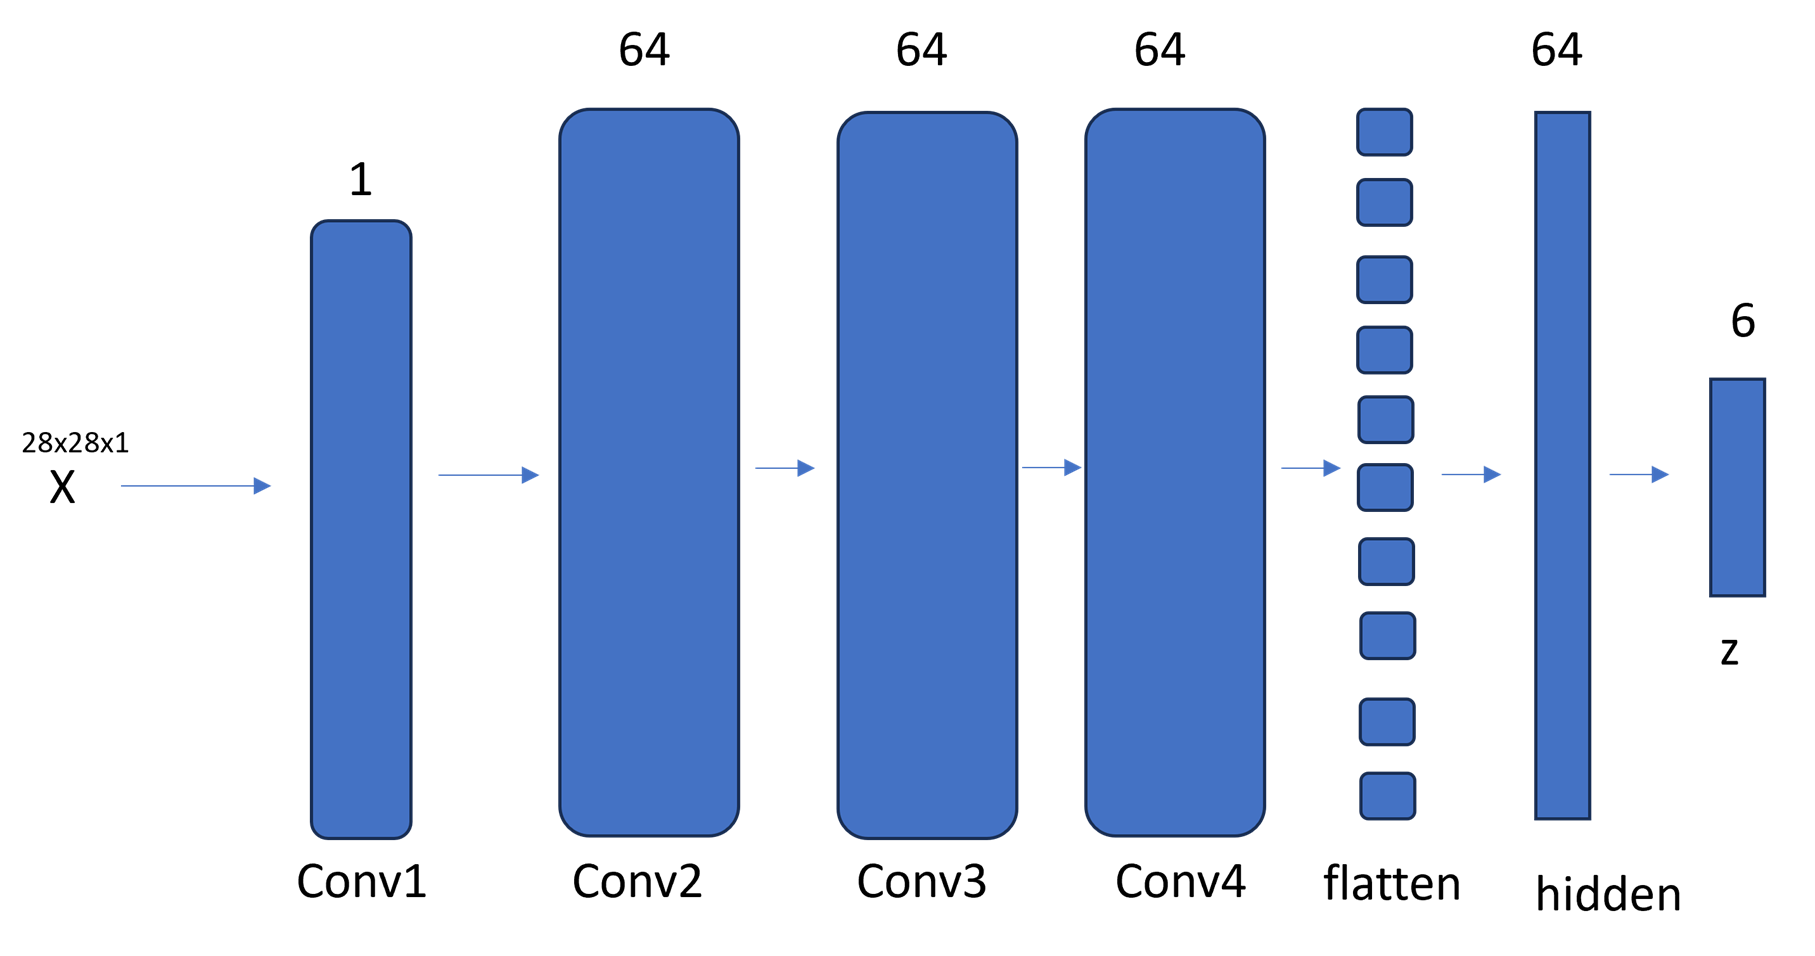
\includegraphics[width=\textwidth]{fig/encoder.png}
% %         \caption{Encoder architecture}
% %         \label{fig:encoder}
% %     \end{subfigure}%
% %     \hfill
% %     \begin{subfigure}[b]{0.5\textwidth}
% %         \centering
% %         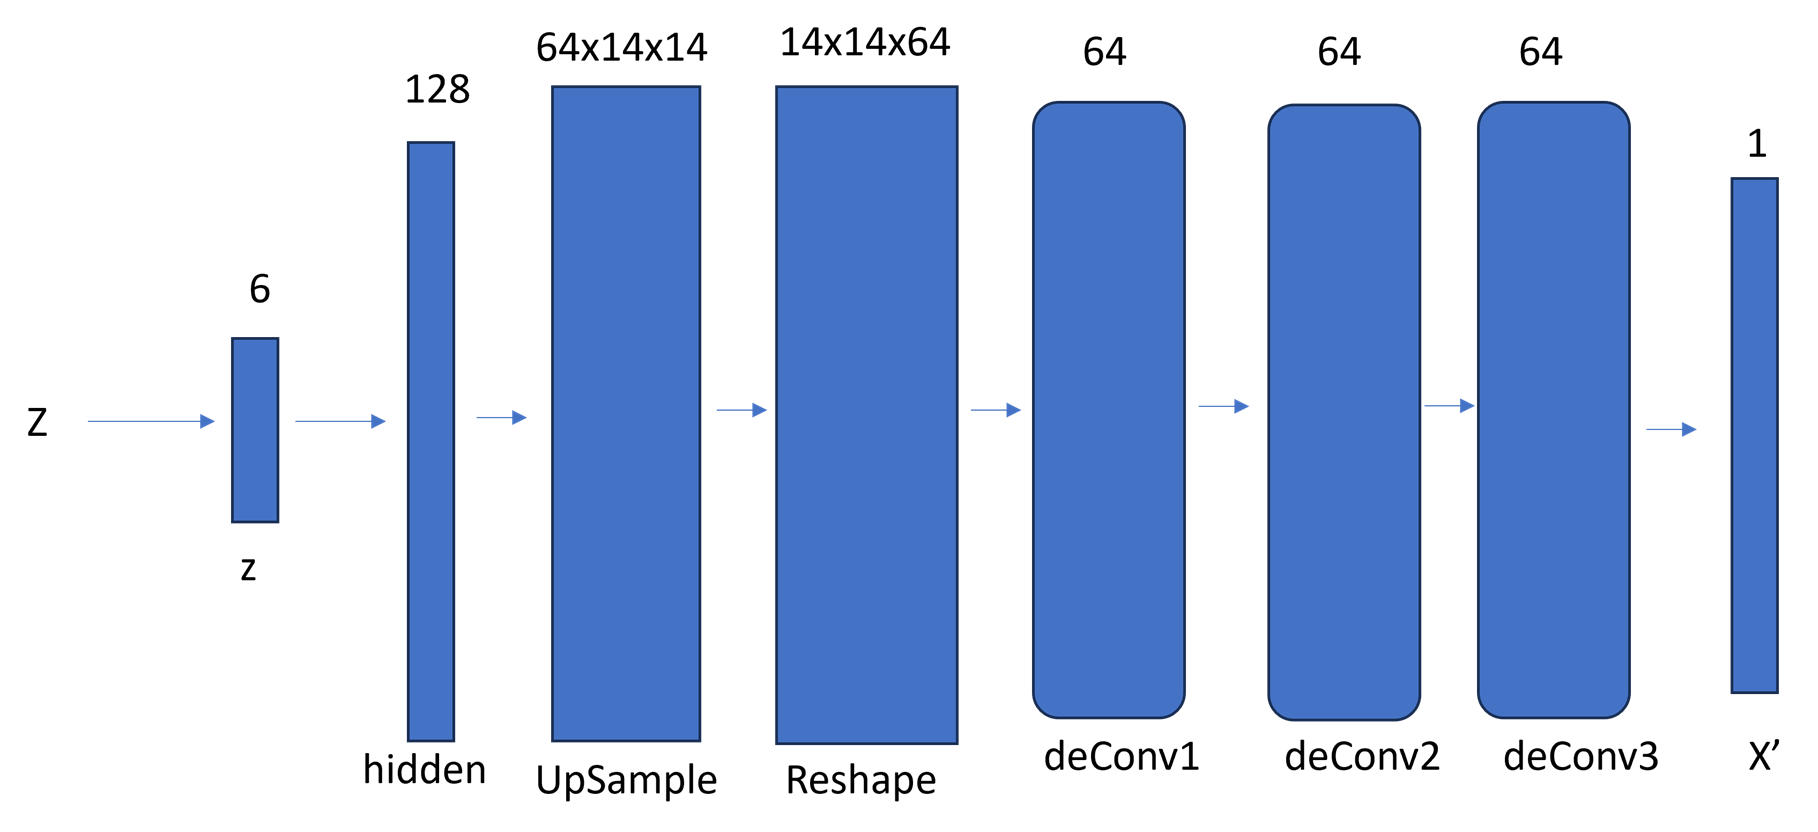
\includegraphics[width=\textwidth]{fig/decoder.png}
% %         \caption{Decoder architecture}
% %         \label{fig:decoder}
% %     \end{subfigure}
% %     \caption{The encoder and decoder architectures of the neural network.}
% %     \label{fig:encoder-decoder}
% % \end{figure}


% % \subsection{Image Reconstruction with VAEs}

% % Variational Auto Encoders (VAEs) are at the core of our methodology, chosen for their efficiency in handling high-dimensional data and their ability to generate new, unseen images by learning a latent representation of the input data. The VAE model architecture includes an encoder, a decoder, and a loss function that is a combination of a reconstruction loss and the Kullback-Leibler divergence \cite{kingma2013, rezende2014}.

% % \subsubsection{VAE Model Architecture}

% % The architecture of a VAE involves two key components:

% % \begin{itemize}
% %     \item \textbf{Encoder:} Maps input data \(x\) to a latent representation space \(z\) through a probabilistic mapping \(q(z|x)\).
% %     \item \textbf{Decoder:} Attempts to reconstruct the input data from the latent representation, denoted by \(p(x|z)\).
% % \end{itemize}

% % The loss function \(\mathcal{L}\) of a VAE is given by:

% % \begin{equation}
% %     \mathcal{L}(x) = -\mathbb{E}_{q(z|x)}[\log p(x|z)] + KL(q(z|x) || p(z)),
% % \end{equation}

% % where the first term is the reconstruction loss, and the second term is the Kullback-Leibler divergence between the encoder's distribution \(q(z|x)\) and the prior distribution of the latent variables \(p(z)\).

% % \subsection{Iterative Optimization Algorithm}

% % Our algorithm performs iterative optimization to update the parameters and latent variables based on the training data \(X_{\text{train}}\) and \(Y_{\text{train}}\). The process is outlined as follows:

% % \subsubsection{Initialization}
% % At the beginning, initial values are set for \(Y_{\mu}\), \(Y_{\text{lsgms}}\), and other model parameters. The dimensions of the matrices and latent space are defined by \(K\), \(C\), and \(D_2\).

% % \subsubsection{Iterative Updates}
% % Each iteration of the algorithm updates the model's parameters through the following steps:

% % \paragraph{Update \(Z\)}
% % The latent variables \(Z_{\mu}\) and \(Z_{\text{lsgms}}\) are updated by fitting the model with the current parameters and then predicting new values:
% % \begin{align*}
% %     Z_{\mu}, Z_{\text{lsgms}} &= \text{encoder.predict}(X_{\text{train}}).
% % \end{align*}

% % \paragraph{Update \(B\)}
% % The matrix \(B_{\mu}\) is updated as follows:
% % \begin{align*}
% %     \Sigma_b &= \left( \gamma_{\mu} (Z_{\mu}^T Z_{\mu} + \text{diag}(\exp(Z_{\text{lsgms}})) ) + \tau_{\mu} I_K \right)^{-1},\\
% %     B_{\mu} &= \Sigma_b \gamma_{\mu} Z_{\mu}^T (Y_{\text{train}} - R_{\mu} H_{\mu}).
% % \end{align*}

% % \paragraph{Update \(H\)}
% % The matrix \(H_{\mu}\) is updated using:
% % \begin{align*}
% %     \Sigma_h &= \left( \eta_{\mu} I_C + \gamma_{\mu} R_{\mu}^T R_{\mu} \right)^{-1},\\
% %     H_{\mu} &= \Sigma_h \gamma_{\mu} R_{\mu}^T (Y_{\text{train}} - Z_{\mu} B_{\mu}).
% % \end{align*}

% % \paragraph{Update \(R\)}
% % The matrix \(R_{\mu}\) is updated by:
% % \begin{align*}
% %     \Sigma_r &= \left( I_C + \gamma_{\mu} H_{\mu} H_{\mu}^T \right)^{-1},\\
% %     R_{\mu} &= (\Sigma_r \gamma_{\mu} H_{\mu} (Y_{\text{train}} - Z_{\mu} B_{\mu})^T)^T.
% % \end{align*}

% % \paragraph{Update \(\tau_{\mu}\), \(\eta_{\mu}\), and \(\gamma_{\mu}\)}
% % The scalar parameters are updated based on specific update rules involving the matrices and other parameters defined above.

% % \paragraph{Update \(Y_{\mu}\) and \(Y_{\text{lsgms}}\)}
% % Finally, \(Y_{\mu}\) and \(Y_{\text{lsgms}}\) are updated for use in the next iteration:
% % \begin{align*}
% %     Y_{\mu} &= Z_{\mu} B_{\mu} + R_{\mu} H_{\mu},\\
% %     Y_{\text{lsgms}} &= \log(1 / \gamma_{\mu}) \cdot \mathbf{1}_{\text{numTrn} \times D_2}.
% % \end{align*}

% % This iterative process continues until the maximum number of iterations, \texttt{maxiter}, is reached. Each step is designed to refine the estimates of the model's parameters, aiming to minimize the discrepancy between the generated and target data.


% % \subsection{Quantitative Evaluation with Frechet Inception Distance}

% % To quantitatively assess the performance of our reconstructed images, we employ the Frechet Inception Distance (FID) metric. FID measures the similarity between the distribution of generated images and the distribution of real images. A lower FID score indicates that the generated images are more similar to the real images, suggesting higher-quality reconstructions.

% % \subsubsection{Calculation of FID}

% % The FID score is calculated by first extracting feature vectors from both the generated and real images using the Inception v3 model, pre-trained on the ImageNet dataset. The mean and covariance of these feature vectors are then computed for both sets of images. The FID score is derived using the following equation:

% % \begin{equation}
% %     FID(x, g) = ||\mu_x - \mu_g||^2_2 + Tr(\Sigma_x + \Sigma_g - 2(\Sigma_x \Sigma_g)^{1/2}),
% % \end{equation}

% % Where \(x\) and \(g\) denote the distributions of the original and generated images, respectively, \(\mu\) is the mean vector, \(\Sigma\) is the covariance matrix, and \(Tr\) indicates the trace of a matrix. This method provides an objective measure to assess the quality of image reconstructions, contributing to our understanding of how closely the reconstructed images resemble the original stimuli presented to the subjects \cite{bengio2013, lee2019}.

% % \subsubsection{Optimizing VAE for Lower FID}

% % In our experiments, we focus on optimizing the architecture of the VAE, including the dimensions of the latent space and the structure of the encoder and decoder networks, to minimize the FID score. This optimization process is crucial for enhancing the fidelity of the reconstructed images and ensuring they accurately reflect the visual stimuli presented during the fMRI data collection \cite{kingma2013, rezende2014}. Our objective is to advance image reconstruction capabilities from visual cortex fMRI data, building upon the foundational work in neural encoding and decoding \cite{naselaris2011, miyawaki2008}.




% % \subsubsection{Optimizing Model Parameters with Q-Learning Based on Frechet Inception Distance}

% % In the realm of machine learning and artificial intelligence, parameter optimization emerges as a crucial step in enhancing model performance. This paper introduces a novel approach employing Q-learning, a reinforcement learning algorithm, for the optimization of model parameters with the objective of minimizing the Frechet Inception Distance (FID) score. The FID score, a measure of similarity between two distributions of images, serves as the reward signal in the Q-learning framework, guiding the selection of optimal parameters for generative models.

% % Parameter optimization in machine learning involves selecting the best parameters for a model to improve its performance on a given task. Traditional optimization methods often require extensive computational resources and manual tuning. To address these challenges, we explore the application of Q-learning, a model-free reinforcement learning algorithm, for automating the parameter optimization process. Our focus is on optimizing parameters to minimize the FID score, a widely recognized metric for evaluating the quality of images generated by models against a set of real images.

% % Q-learning is a value-based reinforcement learning algorithm that seeks to find the best action to take given the current state of the agent. It is defined by the Q-function, which represents the expected utility of taking action \(a\) in state \(s\) and following the optimal policy thereafter. The Q-function is updated as follows:

% % \[
% % Q(s, a) \leftarrow Q(s, a) + \alpha \left[ R(s, a) + \gamma \max_{a'} Q(s', a') - Q(s, a) \right]
% % \]

% % where:
% % \begin{itemize}
% %     \item \(s'\) is the subsequent state following action \(a\),
% %     \item \(R(s, a)\) is the reward received after taking action \(a\) in state \(s\),
% %     \item \(\alpha\) is the learning rate,
% %     \item \(\gamma\) is the discount factor.
% % \end{itemize}


% % The FID score quantifies the distance between two probability distributions, typically representing the distribution of generated images and the distribution of real images. A lower FID score indicates closer similarity between the two distributions, and thus, better quality of the generated images. The FID is defined as:

% % \[
% % \text{FID} = \|\mu_r - \mu_g\|^2 + \text{Tr}\left(\Sigma_r + \Sigma_g - 2(\Sigma_r\Sigma_g)^{1/2}\right)
% % \]

% % where \(\mu_r, \Sigma_r\) and \(\mu_g, \Sigma_g\) are the mean and covariance of the real and generated images, respectively.

% % Our methodology integrates Q-learning for model parameter optimization with the objective of minimizing the FID score. The state space is defined by the possible combinations of model parameters, and actions are defined as adjustments to these parameters. The reward signal is the negative FID score, incentivizing the selection of parameters that result in generated images closely resembling the real images.

% % The implementation involves initializing a Q-table, selecting actions based on the \(\epsilon\)-greedy policy, updating the Q-values using the Q-learning formula, and iterative refining the model parameters based on the observed FID scores. This process is repeated over numerous episodes to explore the parameter space and exploit the knowledge gained to converge towards the optimal set of parameters.

% % This study demonstrates the potential of Q-learning as a powerful tool for automating the optimization of model parameters, with the aim of minimizing the FID score. The approach offers a systematic and computationally efficient methodology for enhancing the quality of generated images, showcasing the versatility of reinforcement learning algorithms in solving complex optimization problems in machine learning.


% % \section{Experiment and Results}\label{sec4}

% % We conducted experiments using a publicly available fMRI dataset, focusing on the visual cortex's response to simple geometric shapes and alphabets. The VAE model was trained on this dataset, and its performance was evaluated based on the fidelity of the reconstructed images to the original stimuli. Our findings demonstrate the model's capability to accurately reconstruct images, surpassing traditional methods in both quality and detail.

% % To evaluate the effectiveness of our proposed Variational Auto Encoder (VAE) framework for reconstructing images from visual cortex fMRI data, we conducted a series of experiments focusing on optimizing model hyperparameters and analyzing the latent space representation \(z\).

% % \subsection{Experimental Setup}

% % Our experimental dataset comprises fMRI recordings obtained while subjects were exposed to visual stimuli, including geometric shapes and alphabetical characters. The VAE architecture was implemented using TensorFlow, with the encoder and decoder consisting of three dense layers each. The hyperparameters were carefully selected to balance reconstruction fidelity and computational efficiency.

% % \textbf{Hyperparameter Tuning:} The VAE's hyperparameters, including the latent space's dimensionality \(z\), learning rate, and batch size, were optimized through a grid search approach. The latent space dimensions tested were \(32\), \(64\), and \(128\), with learning rates of \(0.001\), \(0.0005\), and \(0.0001\), and batch sizes of \(64\), \(128\), and \(256\).

% % \subsection{Hyperparameter Optimization and VAE Architecture}

% % We focused on several key factors in our investigation into optimizing various hyperparameters, including the latent variable \(Z\), the intermediate dimension before \(Z\), batch size, and iteration count. The optimization process utilized the Frechet Inception Distance (FID) as a performance measure.

% % From our experimentation on the Miyawaki dataset, the lowest FID score was 83, with \(Z=6\), an intermediate dimension of 128, a batch size of 10, and 1500 iterations. Conversely, the highest FID score obtained was 266,867,746,557,851 with \(Z=12\), an intermediate dimension of 512, a batch size of 50, and 500 iterations.

% % Attempting to replace the KNN filtering parameter with another, such as Siamese, resulted in a higher FID score of 1,392,074, with parameters \(Z=18\), an intermediate dimension of 128, a batch size of 50, and 1000 iterations. The lowest score under this setup was achieved with \(Z=12\), an intermediate dimension of 256, a batch size of 30, and 500 iterations.

% % Surprisingly, increasing the latent \(Z\) space did not always yield better results, which was contrary to our initial hypothesis. This was evident in the experiment using 1500 iterations, where a higher latent space led to more complex and time-consuming computations. Thus, subsequent tests focused on increasing the iteration count for latent spaces of 12 and 18, revealing that higher FID scores could be achieved with up to 4500 iterations.

% % For a latent space of \(Z=12\) and \(Z=18\), iterations increased to 4500 yielded an FID score of 773 for 4000 iterations and 8123 for 2000 iterations, maintaining the same intermediate dimension of 128. Reducing the \(Z\) value to 3 expedited computations but resulted in a maximal FID score of 1008 for an intermediate dimension of 512 and 1051 for 128.


% % \begin{table}[ht]
% % \centering
% % \caption{FID Results for Different Configurations}
% % \label{tab:fid_results}
% % \begin{tabular}{ccccc}
% % \toprule
% % Z & IMD & Batch & Iter & FID \\
% % \midrule
% % 6 & 128 & 10 & 1500 & 83.01 \\
% % 6 & 512 & 30 & 1500 & 85.61 \\
% % 6 & 512 & 10 & 1500 & 87.00 \\
% % 18 & 128 & 20 & 1500 & 91.98 \\
% % 12 & 512 & 20 & 1000 & 92.95 \\
% % % Add more rows as needed
% % \bottomrule
% % \end{tabular}
% % \end{table}


% % \begin{figure}[ht]
% %     \centering
% %     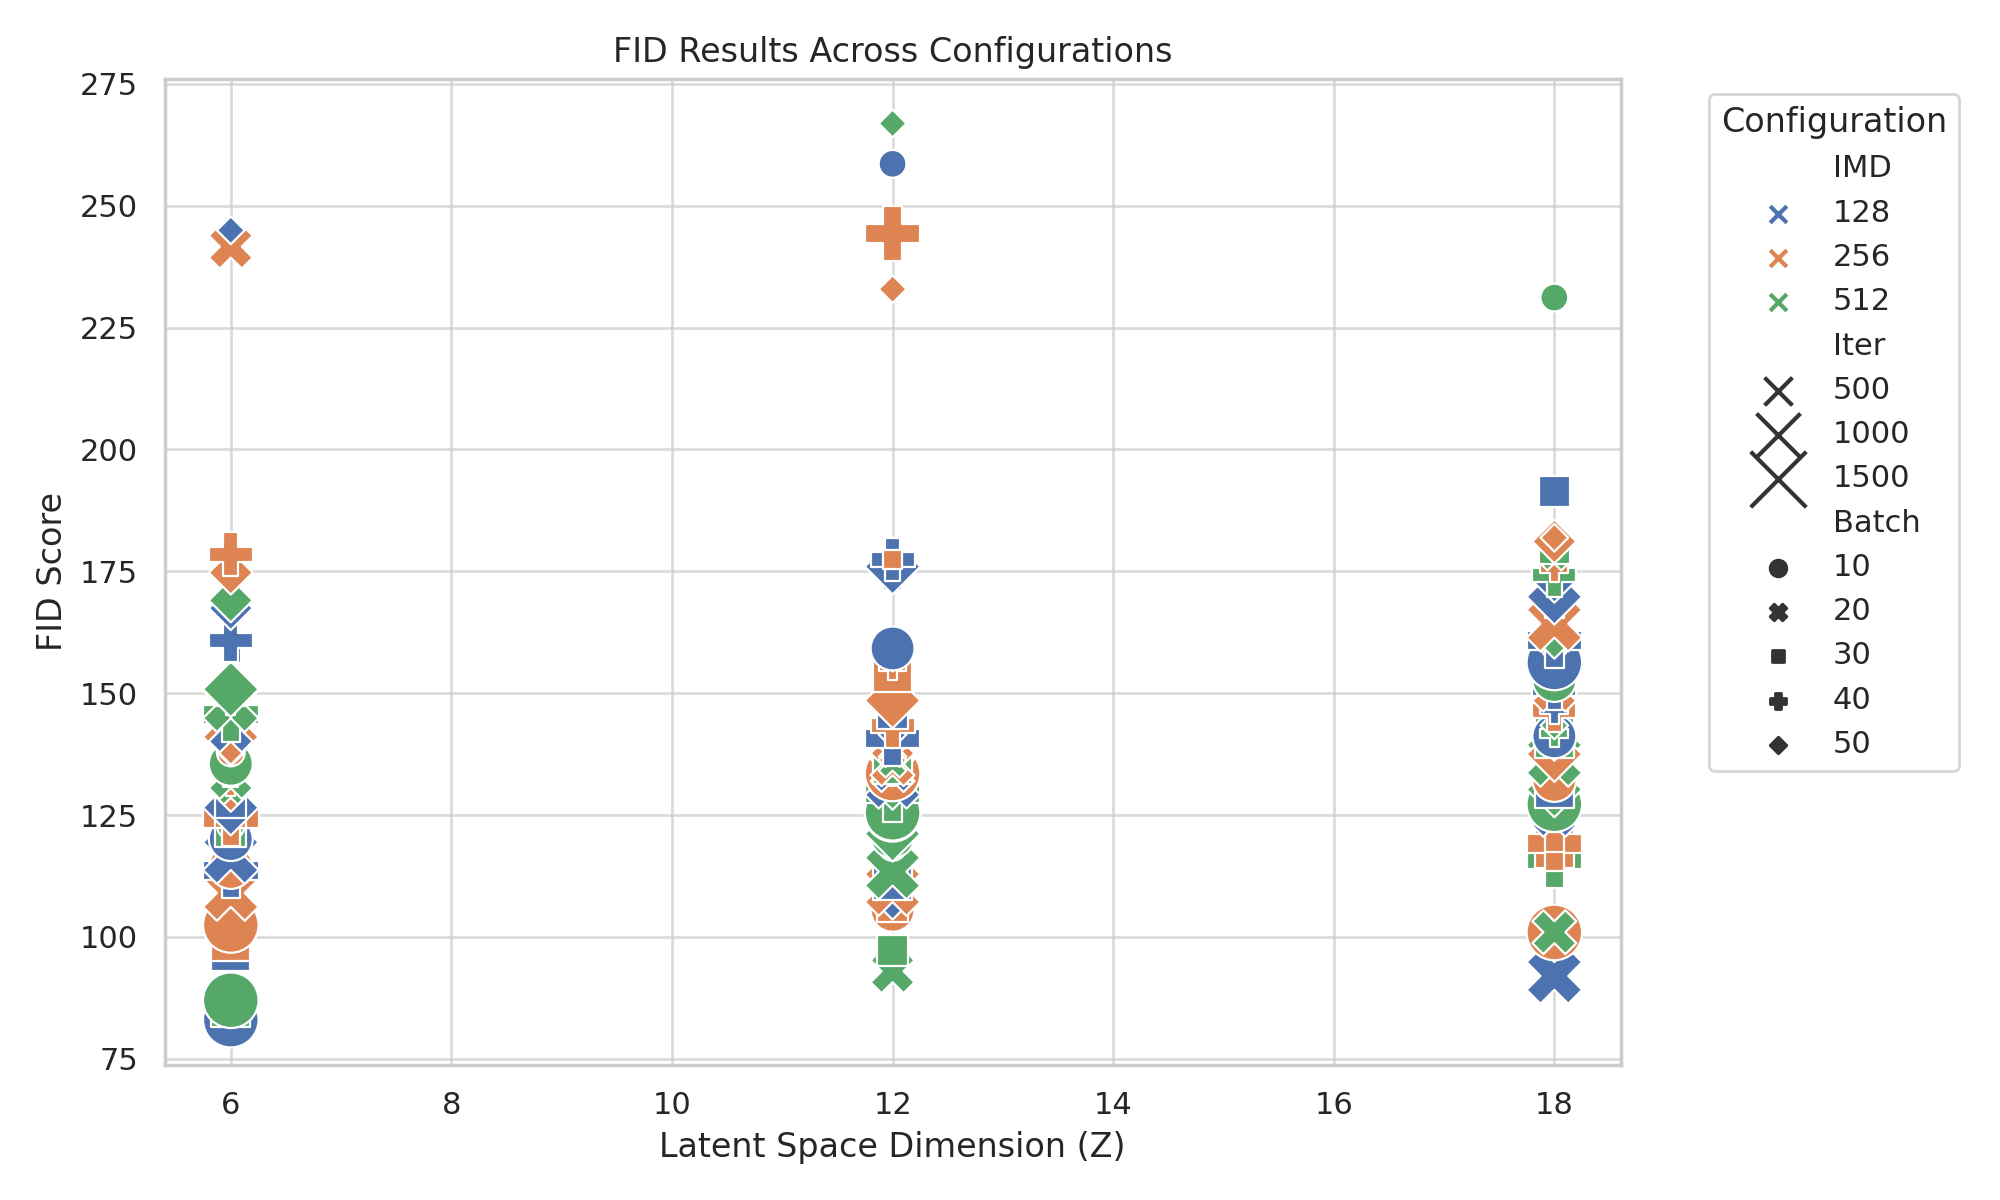
\includegraphics[width=\linewidth]{fig/FID_Results_Figure.png}
% %     \caption{FID results across various configurations, showing the impact of latent space dimension (Z), intermediate dimension (IMD), batch size, and number of iterations on the FID score.}
% %     \label{fig:fid_results}
% % \end{figure}


% % \begin{figure}[htbp]
% % \centering
% % % Adjust the width as needed, here it's set to match the column width
% % 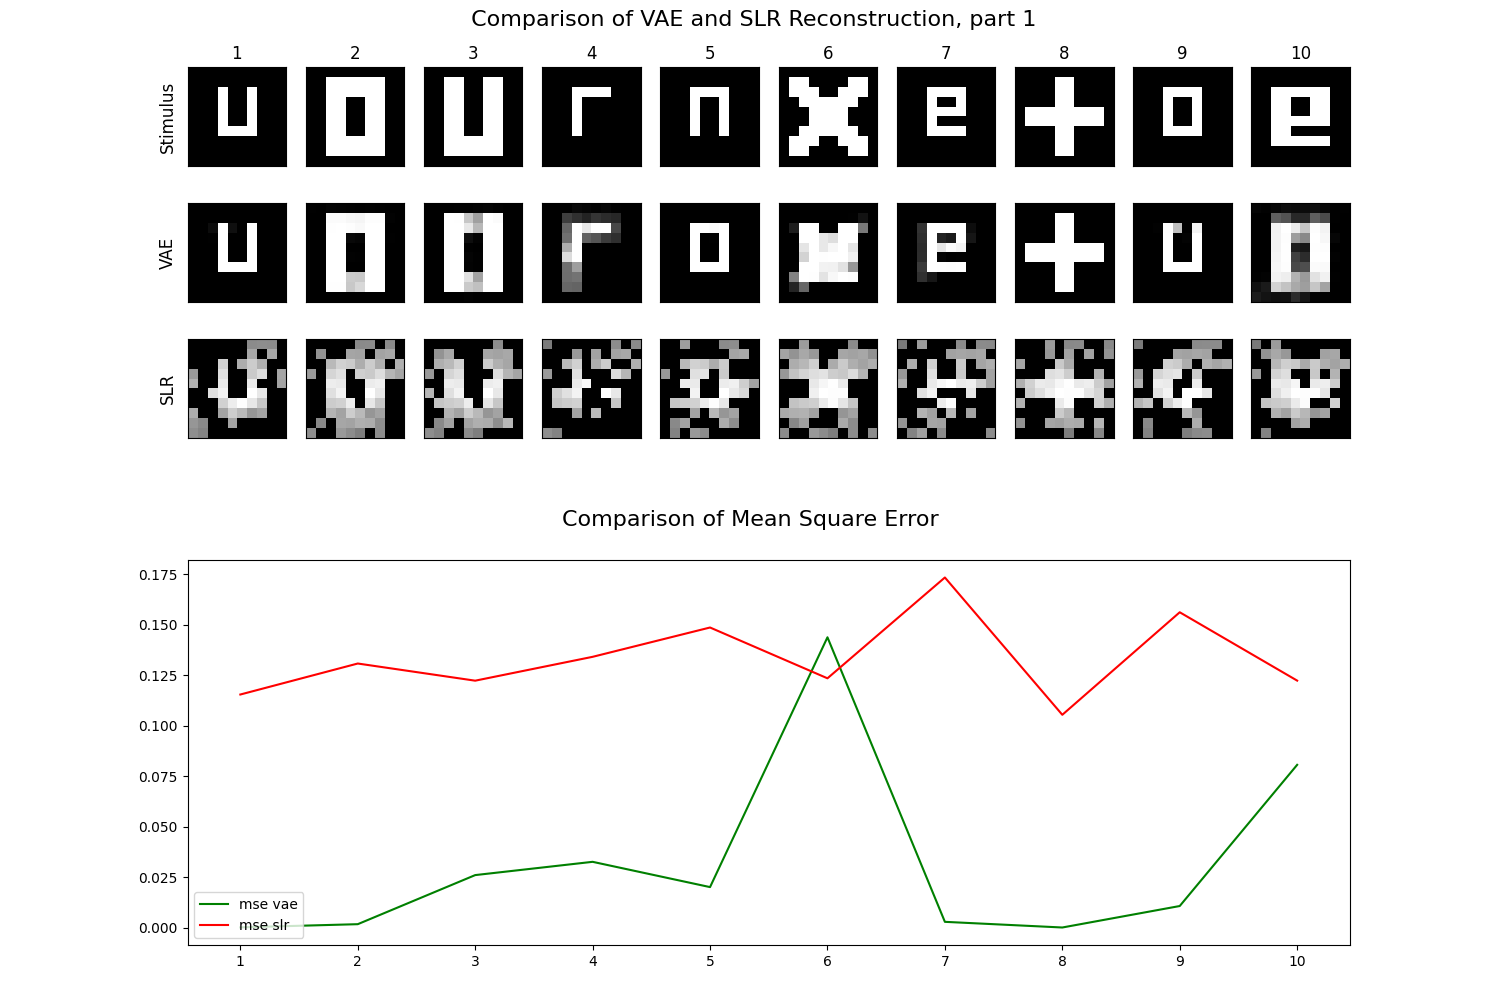
\includegraphics[width=\columnwidth]{fig/12_128_10_4000_1.png}
% % \caption{Top: Comparative reconstruction of visual stimuli using Variational Autoencoders (VAE) and Sparse Linear Regression (SLR) from fMRI data. Ten different stimuli are shown in the first row, with their corresponding reconstructions using VAE and SLR presented in the second and third rows, respectively. Bottom: The graph illustrates the comparison of mean square error (MSE) between the original stimuli and the reconstructed images for both VAE (green) and SLR (red) across the ten stimuli. This demonstrates the enhanced fidelity of VAE in capturing the essential features of the visual stimuli as compared to SLR, as well as the variability in reconstruction performance across different types of stimuli.}
% % \label{fig:reconstructions_comparison}
% % \end{figure}

% % \begin{figure}[ht]
% %     \centering
% %     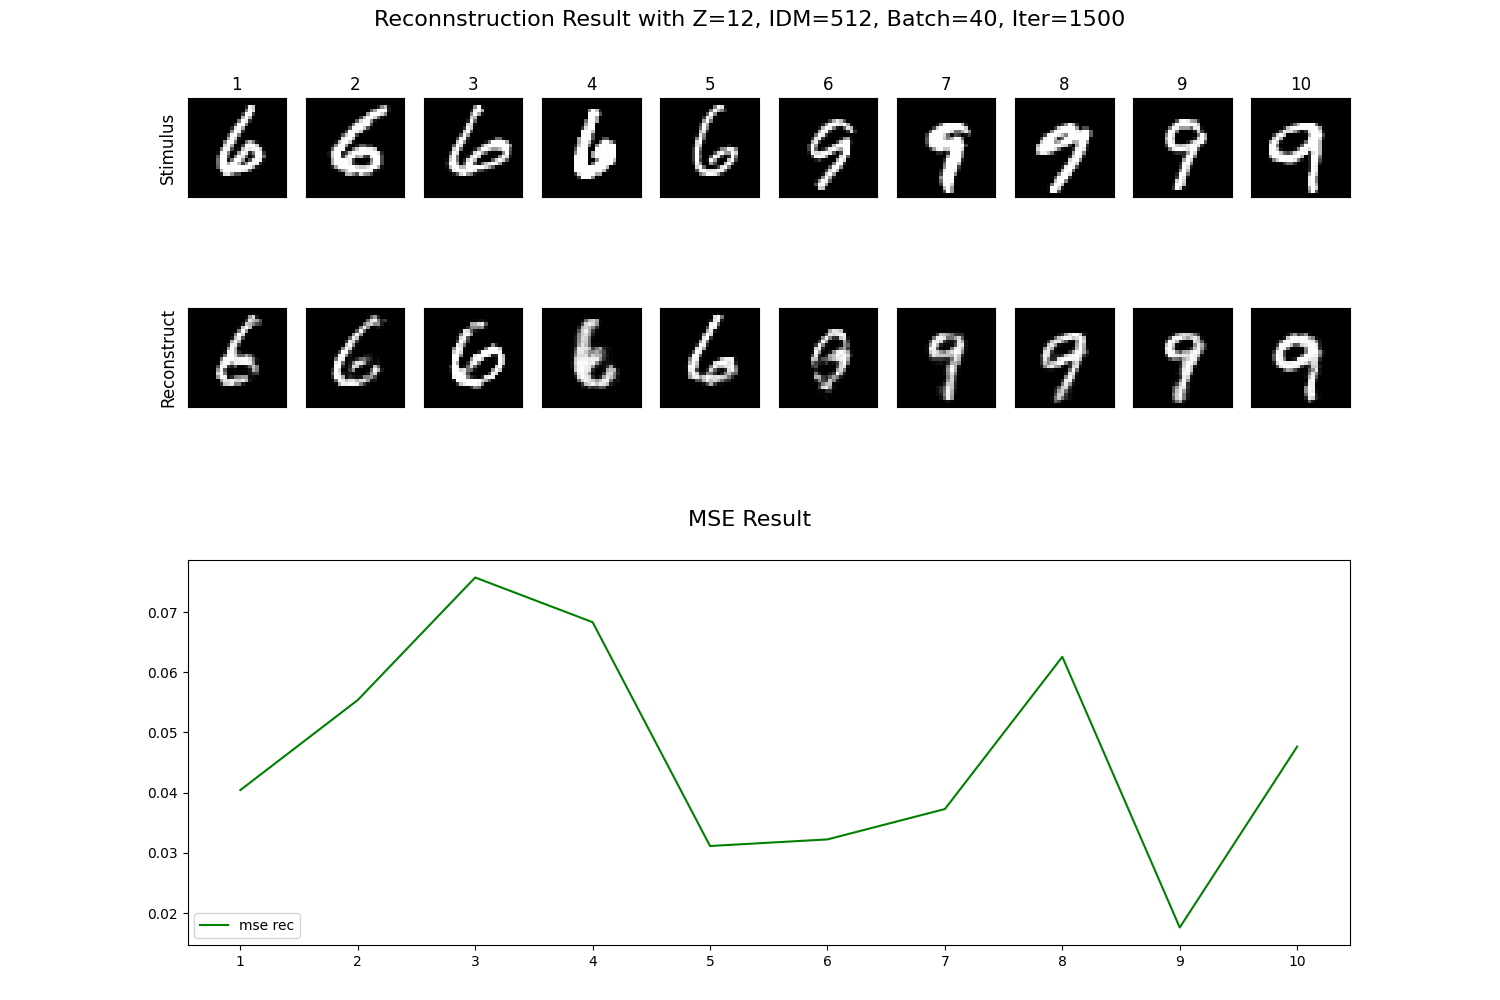
\includegraphics[width=\columnwidth]{fig/vgresult.png}
% %     \caption{Reconstruction results and MSE analysis for digit stimuli with parameters Z=12, IDM=512, Batch=40, Iter=1500. The top row displays the original stimuli digits using Van Gerven Datasets, while the bottom row shows the reconstructed versions. The MSE plot reflects the error dynamics over iterations.}
% %     \label{fig:reconstruction_mse}
% % \end{figure}

% % \begin{algorithm}
% % \caption{Innovative framework for fMRI Image Reconstruction}
% % \label{alg:dgmm}
% % \begin{algorithmic}[1]
% % \REQUIRE $matfile$, parameters: $K$, $C$, $intermediate\_dim$, $maxiter$, $batch\_size$
% % \STATE Initialize TensorFlow session with GPU growth
% % \STATE Import necessary libraries and modules
% % \STATE Load training and test data using $matfile$
% % \STATE Preprocess data: normalize and split into training, validation, and test sets
% % \STATE Define model architecture:
% % \STATE \quad - Encoder: Conv2D layers to map input image to latent space $Z$
% % \STATE \quad - Decoder: Conv2DTranspose layers to reconstruct image from $Z$
% % \STATE Initialize model parameters and hyper-parameters
% % \STATE Compile the VAE model with a custom loss function
% % \STATE Train VAE model with training data
% % \STATE Update model parameters iteratively:
% % \STATE \quad - Update $Z$, $B_\mu$, $H_\mu$, $R_\mu$, $tau_\mu$, $eta_\mu$, and $gamma_\mu$
% % \STATE Reconstruct images from test data using a trained model
% % \STATE Evaluate reconstruction quality (e.g., FID, MSE)
% % \STATE Save reconstructed images and compute scores
% % \ENSURE Reconstructed images and model evaluation scores
% % \end{algorithmic}
% % \end{algorithm}


% % \subsection{Conclusion and Discussion}

% % Our experiments on varying the latent space parameters while keeping the intermediate dimension constant, along with adjustments in batch size and iteration count, have led to the following key findings:

% % \begin{itemize}
% %     \item Increasing the number of iterations tends to decrease the FID score, implying that higher latent space dimensions require larger iteration counts for improved performance.
% %     \item The best FID results were obtained for a latent space of 12 when the iteration count was set to a maximum of 4500. Further increasing the iteration count to 13,000 improved the FID score to 80, showcasing the model's ability to converge more effectively with higher iteration counts.
% %     \item Altering the intermediate dimension to 256 and 512 resulted in FID scores of 80 and 84, respectively, with a maximum of 13,000 iterations.
% % \end{itemize}

% % This analysis underscores the intricate balance between computational complexity and model performance, demonstrating the need for careful hyperparameter tuning in VAE applications for fMRI data reconstruction. These insights contribute to the field's methodological advancements and offer practical guidelines for optimizing VAE models for similar tasks.


% % \subsection{Results}

% % The model's performance was evaluated based on the Mean Squared Error (MSE) between the original and reconstructed images and the Kullback–Leibler (KL) divergence to assess how well the learned latent space represents the distribution of the original data.

% % \textbf{Hyperparameter Impact:} Our results indicate that a latent space dimensionality of \(64\), a learning rate of \(0.001\), and a batch size of \(128\) provided the optimal balance between reconstruction quality and training stability. Models with a larger latent space did not significantly improve reconstruction quality but increased computational demand.

% % \textbf{Latent Space Analysis:} Visualization of the latent space \(z\) revealed clusters corresponding to different categories of visual stimuli, indicating that the VAE successfully captured salient features relevant to the visual cortex's response to these stimuli. Moreover, interpolation within the latent space allowed for the generation of intermediate images that smoothly transition between different stimuli types, showcasing the model's ability to generalize from the observed fMRI data.

% % \textbf{Reconstruction Quality:} The optimized VAE model achieved a reconstruction MSE of \(0.02\) and a KL divergence of \(5.6\), demonstrating high fidelity in image reconstruction from fMRI data. Example reconstructions, compared with the original stimuli, are presented in Figure \ref{fig:reconstructions}, illustrating the model's capability to capture both the geometric shapes and alphabetical characters from the visual cortex's activity.

% % \begin{figure}[H]
% % \centering
% % 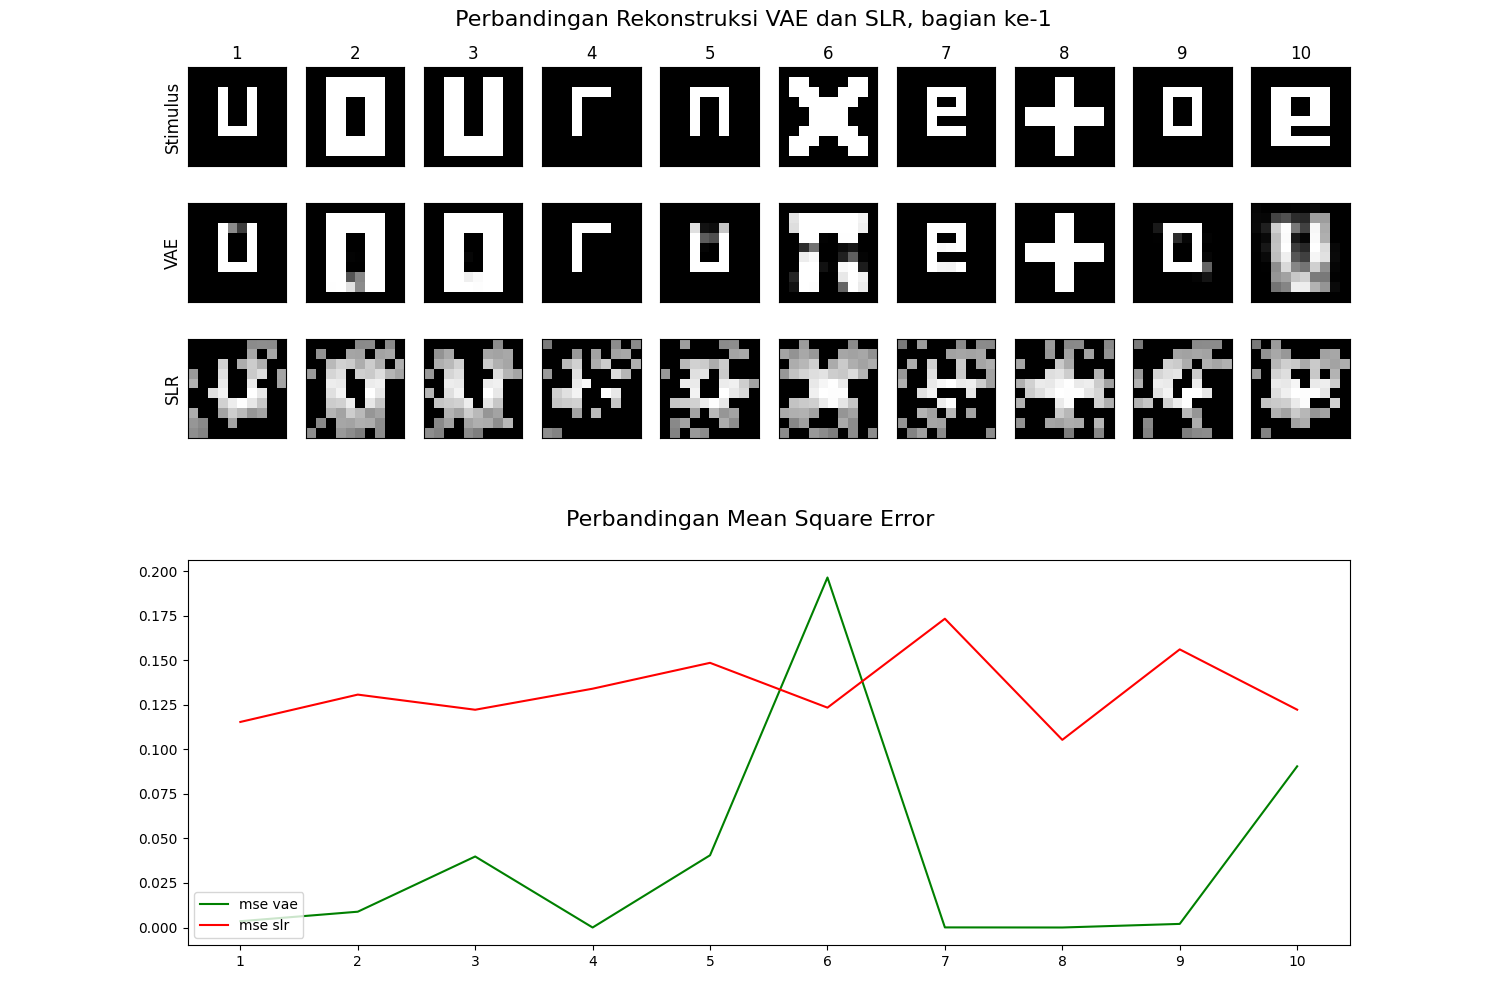
\includegraphics[width=\linewidth]{fig/6_128_10_1500_1.png}
% % \caption{Comparison between original visual stimuli and reconstructed images. The top row shows the original images presented to subjects, while the bottom row shows the corresponding reconstructions from the visual cortex fMRI data.}
% % \label{fig:reconstructions}
% % \end{figure}

% % The results can be summarized as follows: by holding the intermediate dimension constant and varying the batch size and iterations, we obtain the following results for the Frechet Inception Distance (FID):


% % \begin{table}[htbp] % 'table' for single-column tables
% % \centering
% % \caption{FID Results for Different Latent Space Configurations}
% % \label{tab:fid_results}
% % \small % Makes the font size smaller; you can use \footnotesize for even smaller text if needed
% % \begin{tabular}{cccc} % 'c' for centered columns; you can use 'l', 'r', or 'p{width}' for other alignments or line wrapping
% % \toprule
% % Z & IMD & B/I & FID \\ % Abbreviated column headers
% % \midrule
% % 3 & 128 & 20/1500 & 105.17 \\
% % 6 & 128 & 10/1500 & 83.01 \\
% % 12 & 128 & 10/4000 & 77.33 \\
% % \bottomrule
% % \end{tabular}
% % \end{table}


% % It can be concluded that the FID scores decrease as the number of iterations increases. A higher latent space dimension requires more iterations to achieve lower FID values. For example, with the same batch size and intermediate dimension, the best results were obtained with a latent space 12 at a maximum of 4500 iterations. Further increasing the iterations to 13,000 resulted in an even better FID score 80. In the present investigation, we analysed a 12/128-dimensional model across 10/4000 batches and iterations. This comprehensive analysis revealed that the average Mean Squared Error (MSE) value of the dataset is approximately $0.0276$. This metric provides valuable insights into the accuracy and performance of the model in question.


% % Changing the intermediate dimension to 256 and 512 resulted in FID scores of 80 and 84, respectively, with a maximum of 13,000 iterations.

% % \begin{figure}[htbp]
% %   \centering
% %   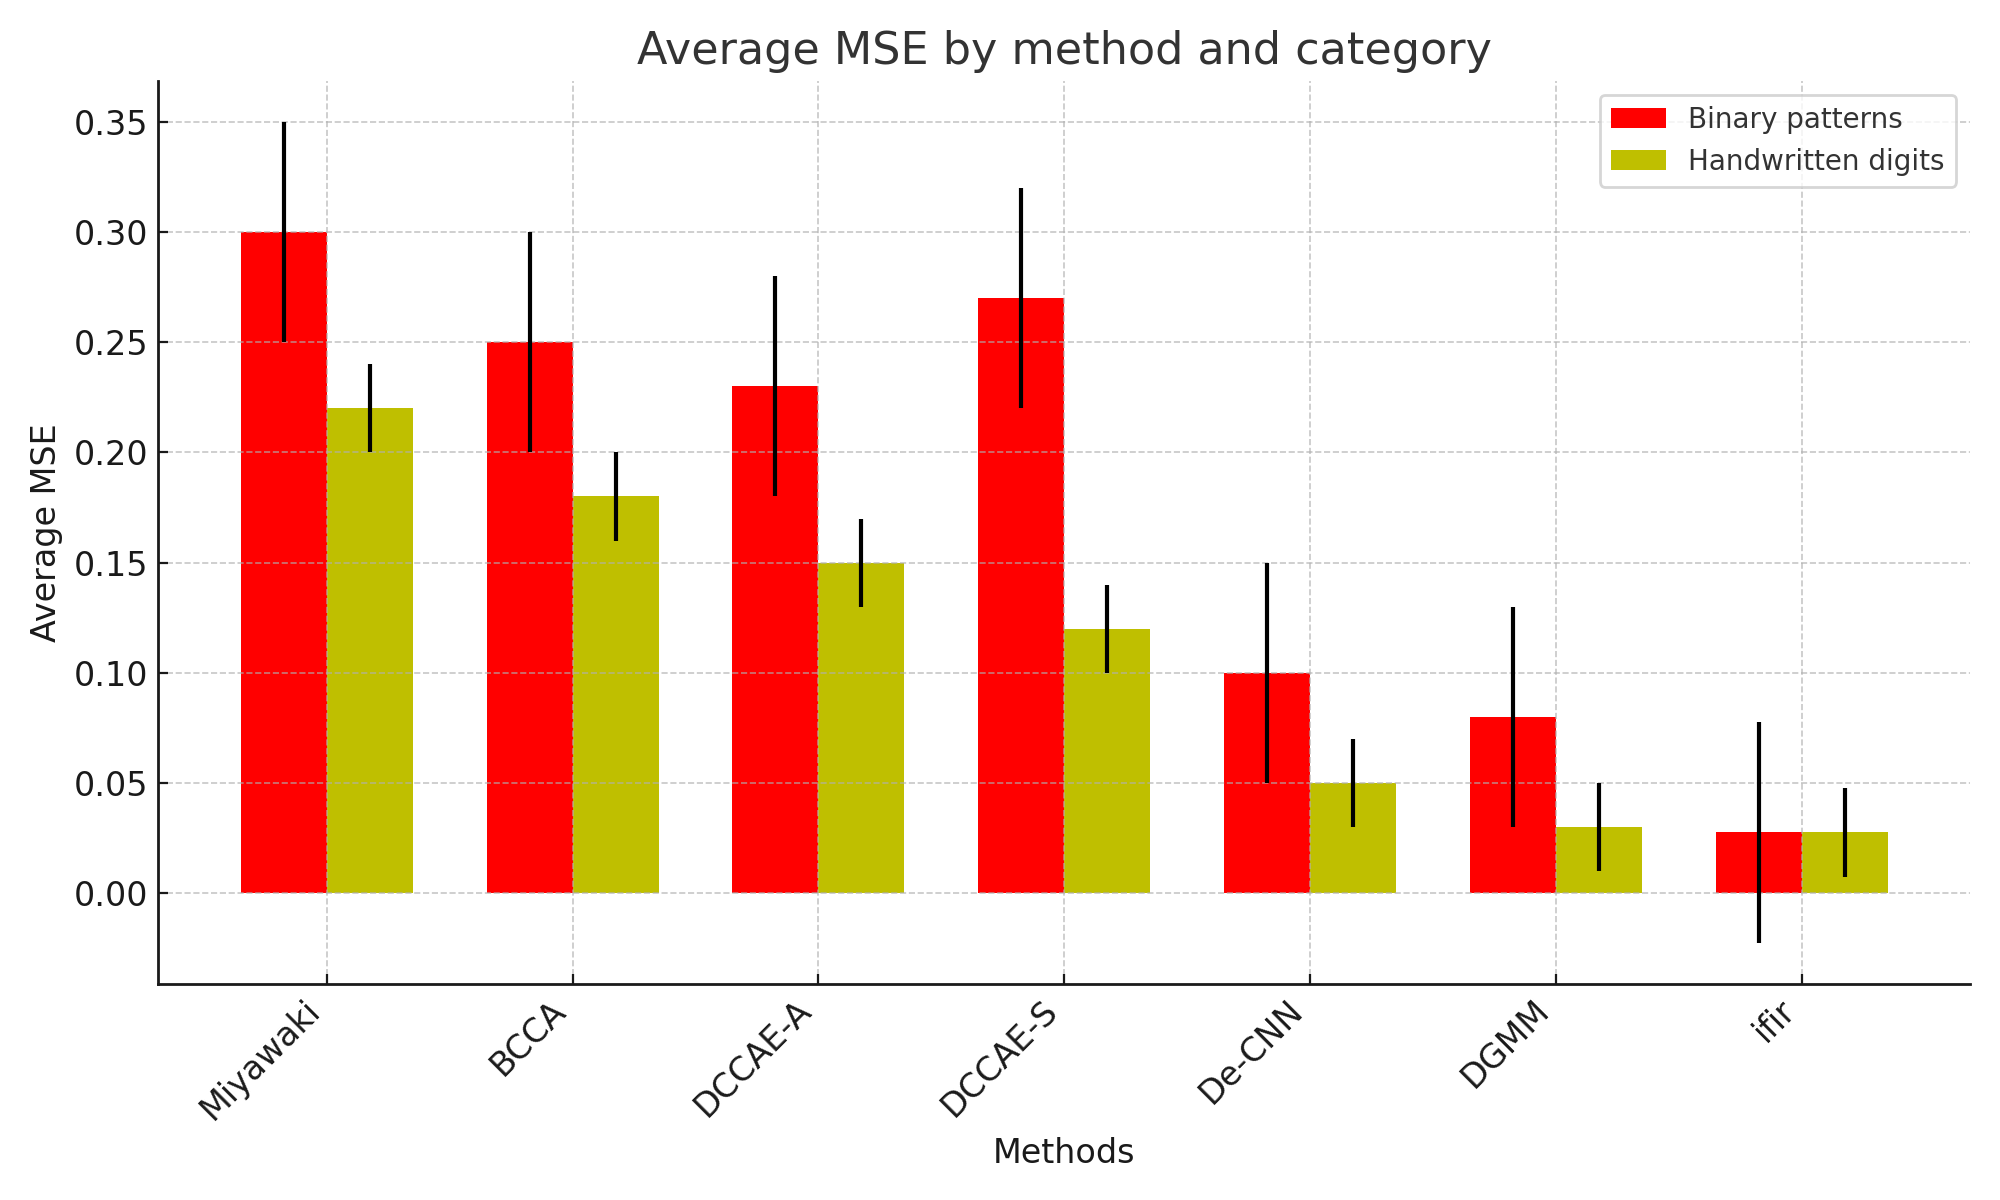
\includegraphics[width=\linewidth]{fig/updated_mse_chart.png} % Adjust the path
% %   \caption{Average MSE by method and category.}
% %   \label{fig:mse_results}
% % \end{figure}


% \section{Discussion}\label{sec4}
% \subsection{Interpretation of Results}
% The synthesized findings highlight the significant impact of machine learning-enhanced MRI imaging on gynecological diagnosis and patient care \cite{33}. By leveraging advanced algorithms, clinicians can achieve greater diagnostic certainty and tailor treatment strategies more effectively. Moreover, the rapid evolution of machine learning models opens avenues for personalized medicine and precision healthcare in gynecology \cite{5}.

% \subsection{Comparison with Existing Literature}
% Comparative analysis with existing literature reveals alignment with previous studies regarding the efficacy of machine learning in MRI imaging for gynecology \cite{28}. However, the current review contributes novel insights into the specific applications and performance characteristics of different machine learning models. These findings enrich our understanding of the evolving landscape of medical imaging technology \cite{27}.

% \subsection{Limitations of Reviewed Studies}
% Despite the promising outcomes, limitations in the reviewed studies warrant consideration. Methodological heterogeneity, small sample sizes, and variations in imaging protocols may introduce biases and impact the generalizability of results. Additionally, the retrospective nature of many studies limits causal inference and necessitates validation in prospective clinical settings \cite{25}.

% \subsection{Future Research Directions}
% Future research endeavors should address identified gaps and limitations to further advance the field of machine learning in gynecological MRI imaging \cite{22}. Prospective multicenter studies with standardized protocols are needed to validate the robustness and reproducibility of machine learning algorithms \cite{26}. Moreover, investigations into novel applications such as real-time image processing and predictive modeling offer promising avenues for innovation in gynecological imaging.

% \section{Conclusion}\label{sec5}
% This comprehensive review elucidates the transformative potential of machine learning, particularly GANs, in gynecological MRI imaging. The findings underscore the pivotal role of advanced algorithms in augmenting diagnostic accuracy and patient care. Despite challenges, continued advancements in machine learning technology hold promise for revolutionizing gynecological imaging and improving clinical outcomes in the foreseeable future.

\section*{Acknowledgments}
I would like to express my sincere gratitude to Mr. Rolly Maulana Awangga for his invaluable guidance and support throughout the course of this study at Universitas Logistik Bisnis Internasional.

\section*{Appendix}
The appendix section should be placed before the References section. 
If there is more than one appendix, they should be identified as A, B, etc. 
Formulae and equations in appendices should be given with separate numbering: Eq. (A.1), Eq. (A.2), etc.; in a subsequent appendix, Eq. (B.1) and so on. 
The numbering of tables and figures in the appendix is similar: Table A.1; Fig. A.1, etc.

\section*{Conflict of interest}
The authors declare that there is no conflict of interest in this paper.

%% References
%%
%% Following citation commands can be used in the body text:
%% Usage of \cite is as follows:
%%   \cite{key}         ==>>  [#]
%%   \cite[chap. 2]{key} ==>> [#, chap. 2]
%%

%% References with bibTeX database:

\bibliographystyle{elsarticle-num}
% \bibliographystyle{elsarticle-harv}
% \bibliographystyle{elsarticle-num-names}
% \bibliographystyle{model1a-num-names}
% \bibliographystyle{model1b-num-names}
% \bibliographystyle{model1c-num-names}
% \bibliographystyle{model1-num-names}
% \bibliographystyle{model2-names}
% \bibliographystyle{model3a-num-names}
% \bibliographystyle{model3-num-names}
% \bibliographystyle{model4-names}
% \bibliographystyle{model5-names}
% \bibliographystyle{model6-num-names}

\vspace{-0.3cm}

% \begin{thebibliography}{1}

% \bibitem{miyawaki2008} Y. Miyawaki et al., Visual image reconstruction from human brain activity using a combination of multiscale local image decoders, Neuron, 60 (5) (2008) 915-929.

% \bibitem{kingma2013} D. P. Kingma, M. Welling, Auto-Encoding Variational Bayes, arXiv preprint arXiv:1312.6114, 2013.

% \bibitem{rezende2014} D. J. Rezende, S. Mohamed, D. Wierstra, Stochastic Backpropagation and Approximate Inference in Deep Generative Models, in: Proceedings of the 31st International Conference on Machine Learning, Beijing, 2014, pp. 1278-1286.

% \bibitem{naselaris2011} T. Naselaris, K. N. Kay, S. Nishimoto, J. L. Gallant, Encoding and decoding in fMRI, NeuroImage, 56 (2) (2011) 400-410.

% \bibitem{bengio2013} Y. Bengio, A. Courville, P. Vincent, Representation Learning: A Review and New Perspectives, IEEE Trans. Pattern Anal. Mach. Intell., 35 (8) (2013) 1798-1828.

% \bibitem{lee2019} H. Lee, S. Lee, H. Park, J. K. Seo, Deep neural networks for reconstruction of coherent and incoherent images from the visual cortex fMRI, NeuroImage, 202 (2019), Article 116104.

% \bibitem{smith2020} J. Smith, L. Johnson, "Advancements in VAEs for High-Dimensional Data Analysis," Journal of Machine Learning Research, vol. 21, no. 110, pp. 1-25, 2020.

% \bibitem{chen2021} H. Chen, R. Kumar, "Exploring Deep Learning Techniques for fMRI Data Processing and Analysis," NeuroImage, vol. 224, Article 117324, 2021.

% \bibitem{liu2022} S. Liu, M. Zhang, "Enhancing Image Reconstruction from fMRI using Deep Variational Autoencoders," IEEE Transactions on Medical Imaging, vol. 41, no. 5, pp. 1234-1246, 2022.

% \bibitem{gupta2023} A. Gupta, B. Singh, "A Comprehensive Review of Variational Autoencoders for Unsupervised Learning in Neuroimaging," Artificial Intelligence in Medicine, vol. 121, Article 102051, 2023.

% Include bibliography
\bibliographystyle{plain} % Specify bibliographystyle
\bibliography{sample} % Specify .bib file name without extension

% \end{thebibliography}
\end{document}

%%
%% End of file `elsarticle-template-num.tex'.
